\documentclass[xcolor=dvipsnames, 14pt]{beamer}
\graphicspath{{./obr/}}
\usetheme[
		%english,
		%nameTitle,
		%tableOfContent,
        %numbering,
        ]{upolkgi}
%%\usetheme{Darmstadt}
%%\usecolortheme[named=LimeGreen]{structure}

% balíčky

%%\usepackage[utf8]{inputenc}
%%\usepackage[czech]{babel}
\usepackage{graphicx}

% informace o dokumentu
 \setbeamersize{text margin left=.5cm,text margin right=.5cm, text margin top=2cm}
 \pdfcompresslevel=0
\begin{document}

\title[Synchronizace a replikace geodat]{Synchronizace a replikace geodat \\v prostředí Esri platformy}
\author[M. Solanská]{Markéta Solanská \\vedoucí práce doc. RNDr. Vilém Pechanec, Ph.D.}
\date[6.3.2013]{3. diplomový den, 26.3.2014}

% titulní stránka
% (název prezentace, autor, datum...)

\begin{frame}
  \titlepage
\end{frame}

\section{Synchronizace a replikace geodat v prostředí Esri platformy}

  \begin{frame}
    \frametitle{Cíle práce}
    \begin{itemize}
        \item nastudovat možnosti ArcSDE a vyzkoušet připojení dat z databáze PostgreSQL k produktům ArcGIS
        \item nastudovat a prakticky otestovat možnosti replikace dat mezi PostgreSQL servery, její typy a nastavení
    \end{itemize}
  \end{frame}
  
  \begin{frame}
    \frametitle{Princip replikace}
    \centering
    
\includegraphics[scale=0.45]{obr/schema1.png} 
  \end{frame}

  \begin{frame}
    \frametitle{Princip replikace}
    \centering
    
\includegraphics[scale=0.45]{obr/schema1-sde.png} 
  \end{frame}

  \begin{frame}
    \frametitle{Princip replikace}
    \centering
    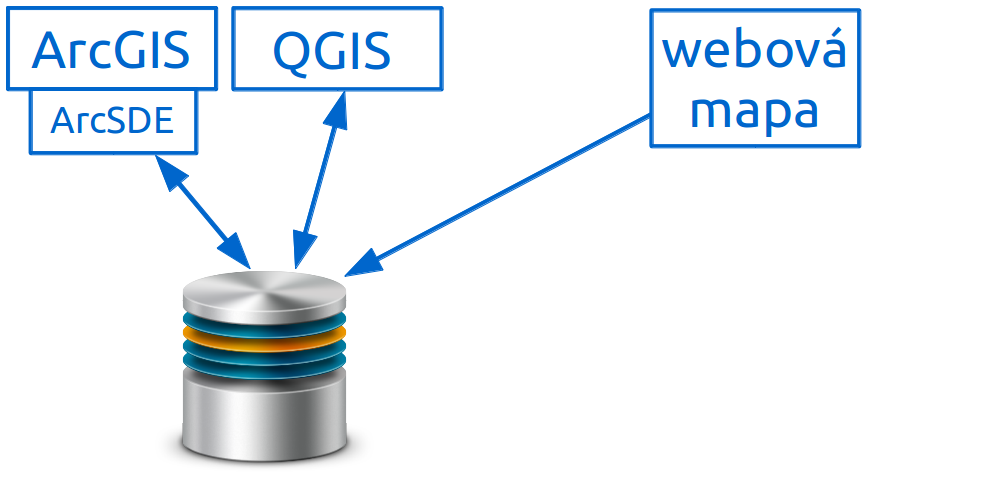
\includegraphics[scale=0.45]{obr/schema2.png} 
  \end{frame}

  \begin{frame}
    \frametitle{Princip replikace}
    \centering
    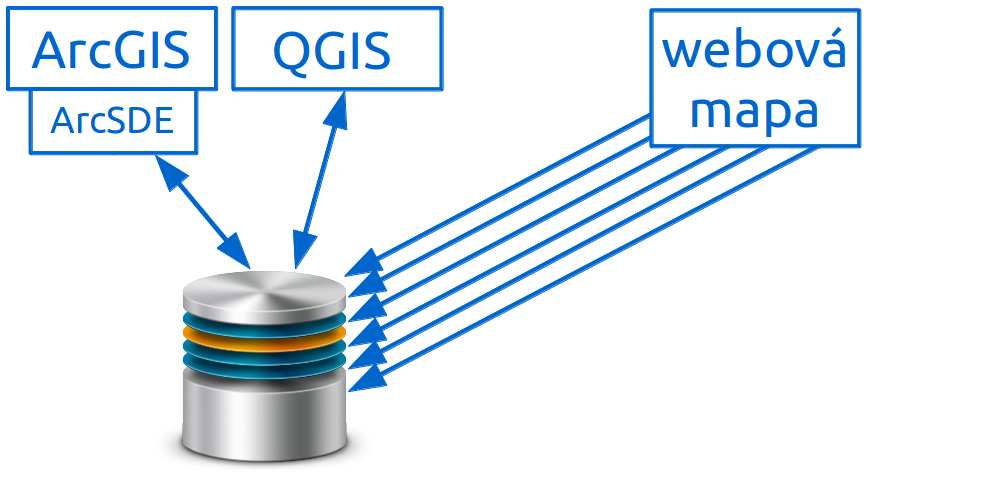
\includegraphics[scale=0.45]{obr/schema3.png} 
  \end{frame}

  \begin{frame}
    \frametitle{Princip replikace}
    \centering
    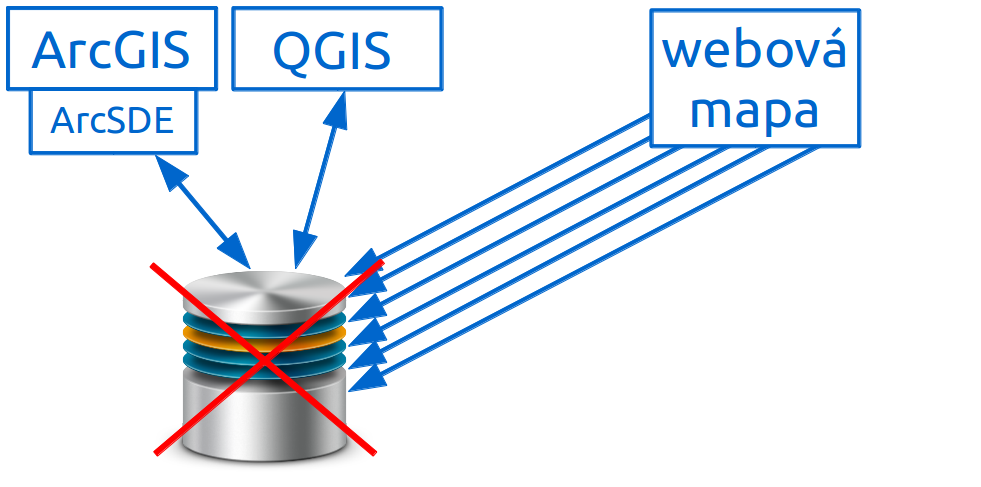
\includegraphics[scale=0.45]{obr/schema4.png} 
  \end{frame}

  \begin{frame}
    \frametitle{Princip replikace}
    \centering
    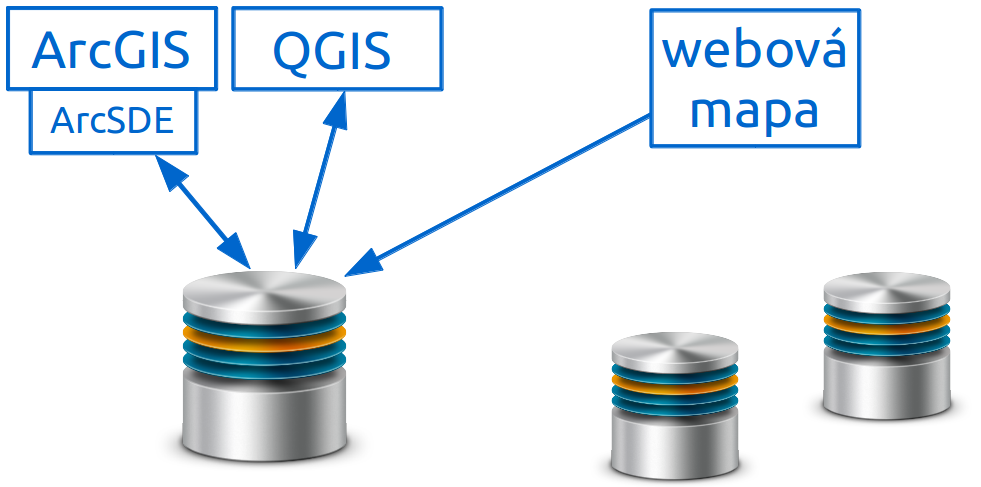
\includegraphics[scale=0.45]{obr/schema5.png} 
  \end{frame}

  \begin{frame}
    \frametitle{Princip replikace}
    \centering
    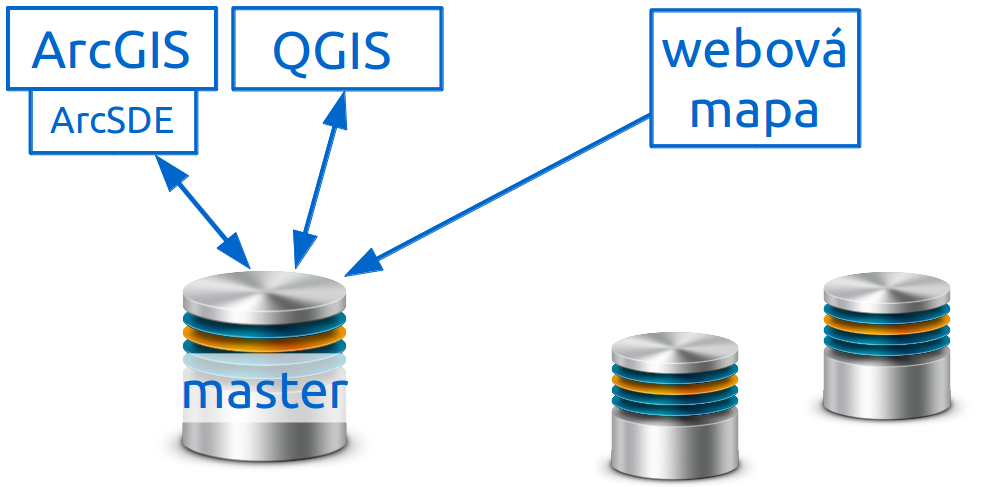
\includegraphics[scale=0.45]{obr/schema6.png} 
  \end{frame}

  \begin{frame}
    \frametitle{Princip replikace}
    \centering
    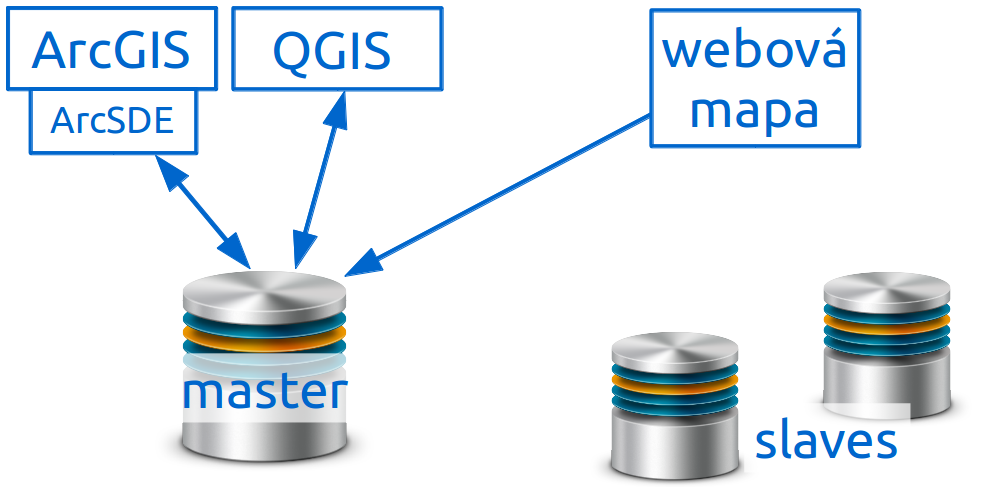
\includegraphics[scale=0.45]{obr/schema7.png} 
  \end{frame}

  \begin{frame}
    \frametitle{Princip replikace}
    \centering
    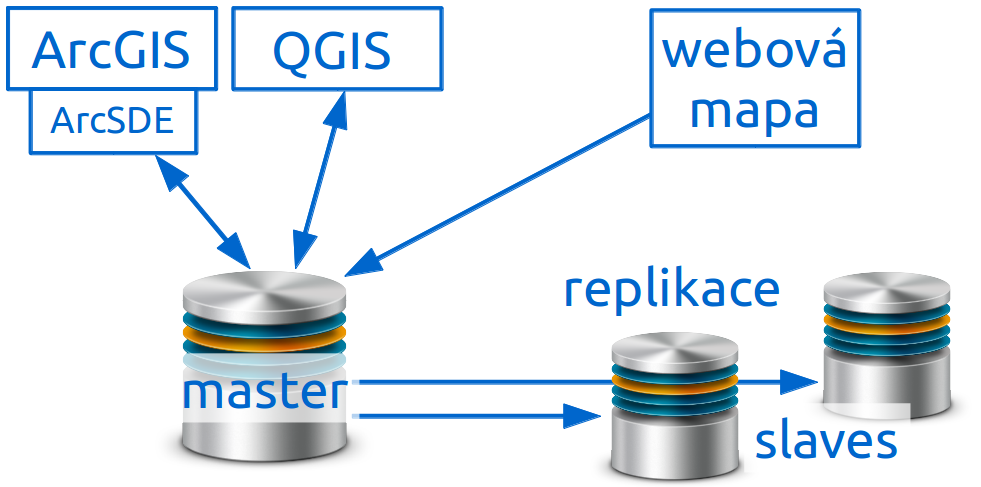
\includegraphics[scale=0.45]{obr/schema8.png} 
  \end{frame}

  \begin{frame}
    \frametitle{Princip replikace}
    \centering
    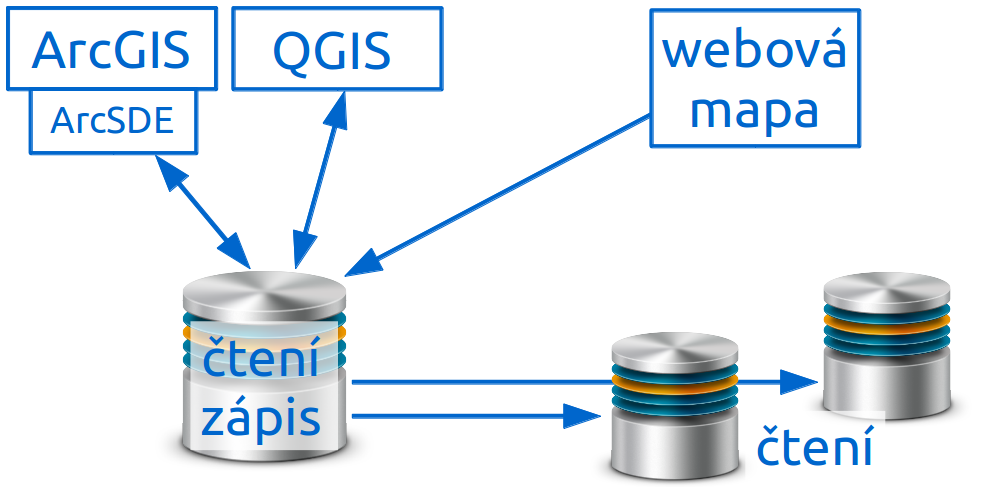
\includegraphics[scale=0.45]{obr/schema9.png} 
  \end{frame}

  \begin{frame}
    \frametitle{Princip replikace}
    \centering
    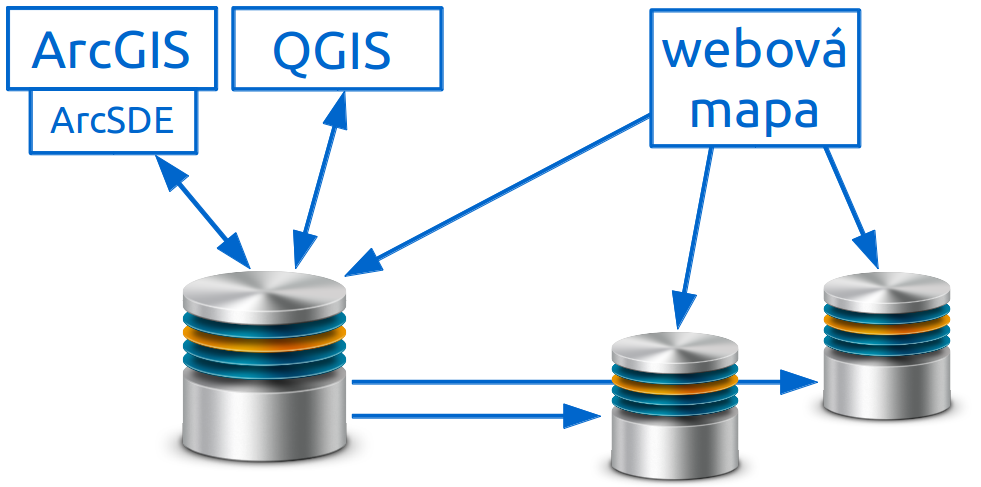
\includegraphics[scale=0.45]{obr/schema10.png} 
  \end{frame}

  \begin{frame}
    \frametitle{Princip replikace}
    \centering
    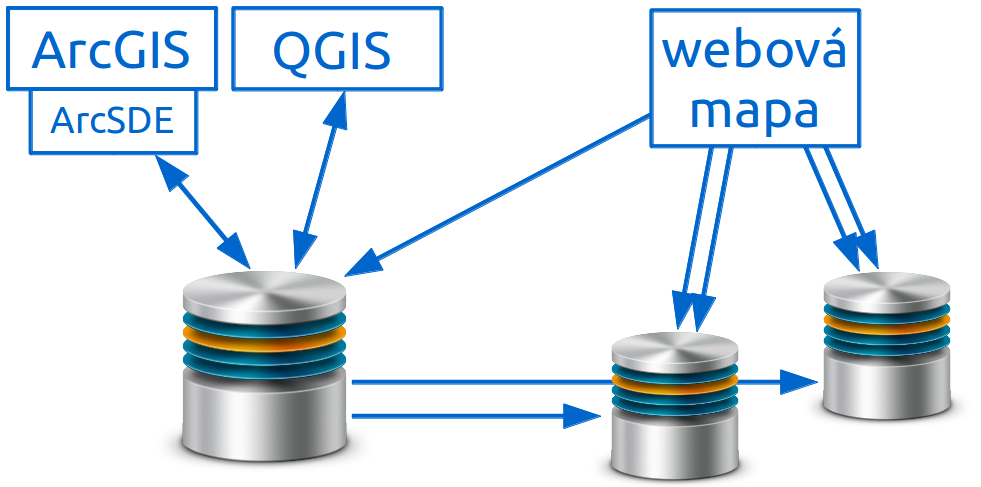
\includegraphics[scale=0.45]{obr/schema11.png} 
  \end{frame}

  \begin{frame}
    \frametitle{Princip replikace}
    \centering
    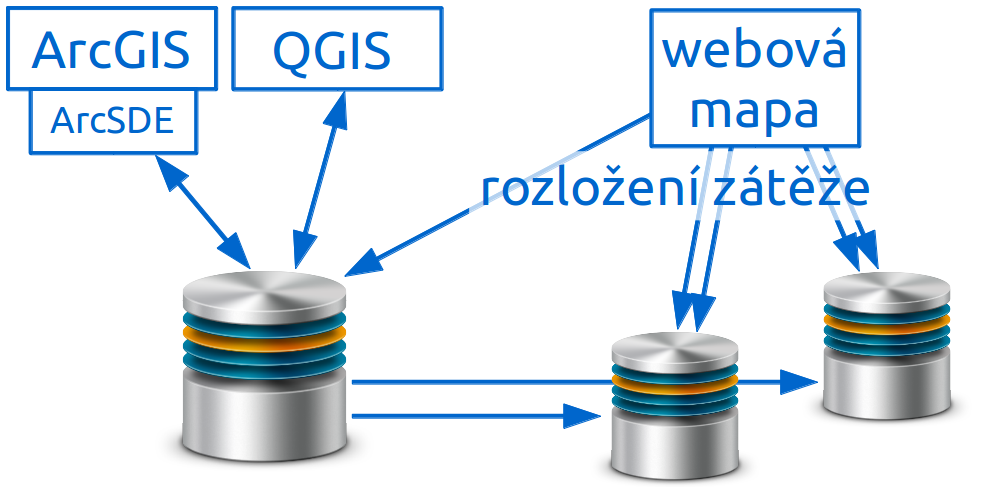
\includegraphics[scale=0.45]{obr/schema12.png} 
  \end{frame}

  \begin{frame}
    \frametitle{Princip replikace}
    \centering
    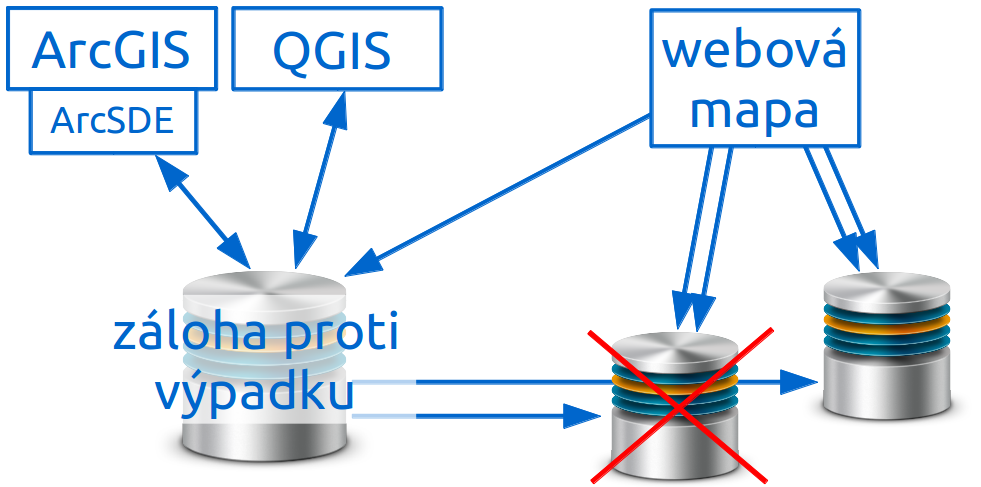
\includegraphics[scale=0.45]{obr/schema13.png} 
  \end{frame}

  \begin{frame}
    \frametitle{Princip replikace}
    \centering
    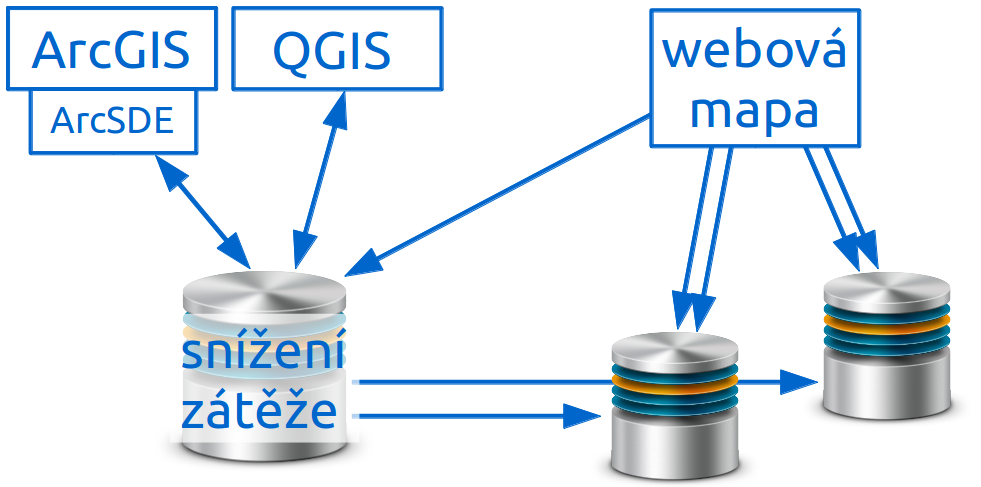
\includegraphics[scale=0.45]{obr/schema14.png} 
  \end{frame}

  \begin{frame}
    \frametitle{Již hotovo}
    \begin{itemize}
      \item studium procesu replikace a fungování ArcSDE
      \item teoretická a rešerší část
      \item praktické použití 2 typů replikace PostgreSQL
          \begin{itemize}
            \item Slony-I replikace (na WIN XP/Linux Ubuntu)
            \item built-in replikace (na Linux Ubuntu)
          \end{itemize}
    \end{itemize}
  \end{frame}

  \begin{frame}
    \frametitle{Co bude brzy hotovo}
    \begin{itemize}
      \item praktické otestování ArcSDE, jeho verzování a replikace
      \item testování replikace na velkém objemu dat
      \item dokončení textové části práce
    \end{itemize}
  \end{frame}

  \begin{frame}
    \hspace*{2em}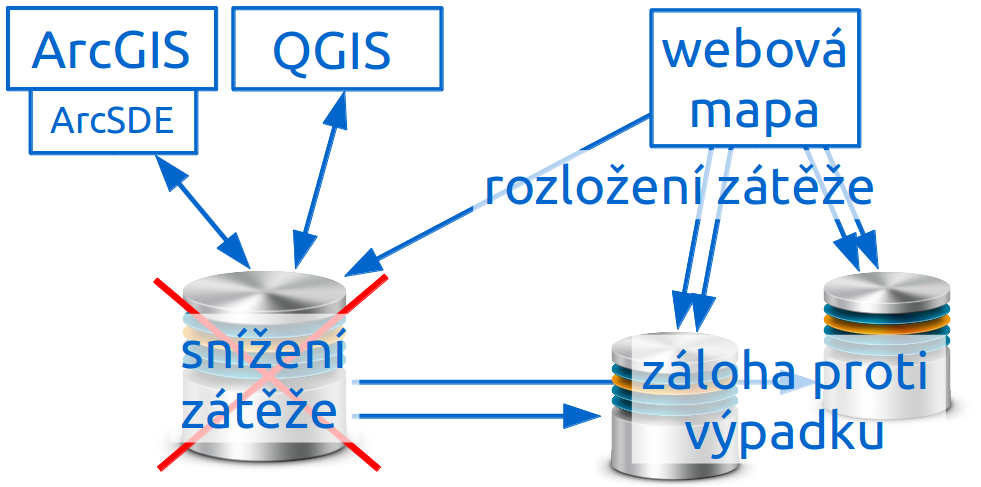
\includegraphics[scale=0.3]{obr/schema_zaver.png} 
      \vspace{30px}
      \newline\centering{\LARGE\color{GisLightBlue}Děkuji za pozornost.}
      
  \end{frame}
\end{document}
